\section{Classical Molecular Dynamics}

\subsection{Introduction}

Ab initio (DFT) calculations approximately solve the schrodinger equation to calculate the energy, forces and stress of a given simulation.  They take a relatively long time to calculate, have relatively small numbers of atoms (hundreds to thousands) and are fixed at one moment in time, although there are now programs that will run DFT MD.  In comparison, Molecular Dynamics model a collection of atoms over a specified period of time.  Much larger collections of atoms are possible (thousands to millions) and the interaction between atoms are predefined by interatomic potentials.




\subsection{Neighbour List}





\subsection{Verlet Timestep}


\begin{itemize}
\item Build a neighbourlist
\item Calculate the force on each atom
\item Start loop with a time step $\Delta t$
\item Calculate the half time step velocity $\vec{v}(t+0.5 \Delta t) = \vec{v}(t) + 0.5 \Delta t \times a (t)$
\item Using the half time step velocity, move the atoms to their new position
\item Update or rebuild the neighbour list
\item Recalculate the forces (and acceleration) at time $t+\Delta t$
\item Calculate the end velocity

\ldots 
\end{itemize}



\subsection{Selecting a Time Scale}

Take, for example, a 50x50x50 BCC Iron supercell with a lattice parameter of 2.87 angstrom.  The supercell measures almost 15nm on each side.  Simulating a thermal neutron, travelling at 2,200 m/s, would require an overall time period of at least 7 picosecond to capture the neutron passing through the supercell.  Higher energy particles would require smaller overall time periods, divided up into as many time steps as the user requires.  

If PKA damage is being modelled, there may be a point where the depth of the damage cascade becomes larger than the supercell itself.  Damage cascades of 500KeV iron atoms into an iron target travel to a depth of up to 300nm, which would require a simulation supercell at least 1,000 BCC cells deep.  Kinetic Monte Carlo would be better suited at simulating higher energy damage cascades.   

\begin{figure}[h]
  \begin{center}
    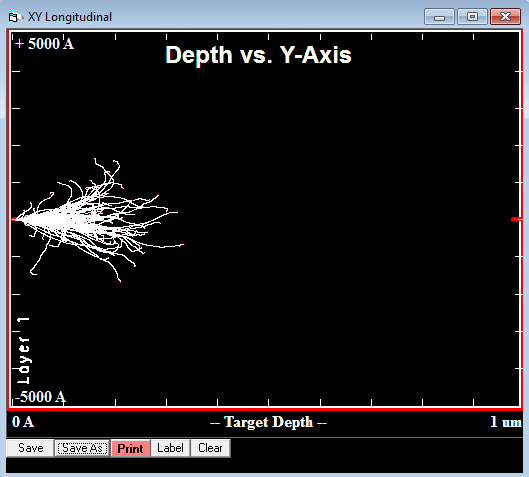
\includegraphics[scale=0.70]{chapters/background_potential_fitting/plots/fe500kev.png}[scale=0.6]
    \caption{Damage cascade: 500kev iron projectiles into an iron target calculated with SRIM}
    \label{graph:fe500kev}
  \end{center}
\end{figure}




